% !TEX TS-program = make

%
% report.tex: The source code for the NPS report
%
\documentclass[report,singlespace,times,makeidx]{npsreport}

%
% Packages we are using
%
\usepackage[T1]{fontenc}
\usepackage{textcomp}
\usepackage{url}
\usepackage{pdfpages}
% Hyperref adds PDF metadata
% TAKE THIS OUT if it causes problems.
% Specifically, remove if you are using xelatex
\usepackage[pdftex,
  pdftitle={\@title}, 
  pdfauthor={\@author},
  pdfpagemode=UseOutlines,
  bookmarks=true,
  colorlinks=false]{hyperref}	% understand PDF refs
\usepackage[all]{hypcap}             % must follow hyperref

%
% Need multiple indices
%    http://mirror.math.ku.edu/tex-archive/macros/latex/contrib/splitindex/splitidx.pdf
%
\usepackage{splitidx}                % pkg for multiple indices
\makeindex                           % we want an index
\newindex[Student Index]{student}    % first index
\newindex[Faculty Index]{faculty}    % second index


%
% Macros
%
\DefineShortVerb{\|}                 % makes |foo| a verbatim command
\renewcommand{\ttdefault}{pcr}       % Allow the courier to be made bold

\newcommand{\graddate}{December 2004}

\POReportNumber{NPS-04-11-00X}
\title{Compilation of\\ THESIS ABSTRACTS}
\author{Office of the Vice President and Dean of Research}

%
% Derivative information
%
\date{\graddate}              % use graduation date



            % a bunch of macros for this report
% custom macros for NPS Report

\newcommand{\npsrsectdegree}[1]{
  \newpage
  \part*{\textsc{#1\xspace}}
  \addcontentsline{toc}{part}{#1\xspace}
  \renewcommand{\leftmark}{#1\xspace}
  \thispagestyle{plain}
  
}

% #1  long version - display on page
% #2  short version - for TOC
\newcommand{\npsrsectfield}[2]{
  \newpage
  \chapter*{\textsc{#1\xspace}}
  \addcontentsline{toc}{chapter}{#2\xspace}
  \thispagestyle{plain}
  
}

\newcommand{\npsrtitle}[1]{
  \addcontentsline{toc}{section}{#1\xspace}
  \begin{center} \textsc{\textbf{#1\xspace}}\\           % end in npsrabstract
}

\newcommand{\npsrauthor}[2]{
  \textbf{#1\xspace}\sindex[student]{#2}\xspace
}

\newcommand{\npsrauthorservice}[1]{
  --- \textbf{#1\xspace}\\
}

\newcommand{\npsrdegree}[1]{
  \textbf{#1\xspace}\xspace
}

\newcommand{\npsrdegreedate}[1]{
  --- \textbf{#1\xspace}\\
}

\newcommand{\npsradvisorbegin}{
  \textbf{Advisor: }
}
\newcommand{\npsradvisorsbegin}{
  \textbf{Advisors: }
}

\newcommand{\npsradvisors}[2]{
  \textbf{#1\xspace}\sindex[faculty]{#2}\xspace
}

\newcommand{\npsrabstract}[1]{
  \\\end{center} #1 \vspace{5pt}\newline           % end centering of title info
}

\newcommand{\npsrkeywords}[1]{
  \textsc{Keywords:} #1 \\
}

\newcommand{\npsrurl}[1]{
  {\sc Available on Calhoun at:} \url{#1} \\ \\
}

    % a bunch of macros for typesetting calhoun data

%
% Begin the document
%
\begin{document}

\abstract{}                   % this is necessary, for some reason
\NPSabstractWasPrintedtrue    % we don't want an abstract, though
\NPScoverOld                  % variant cover

%
% Style the pages
%
\chead{\bf \leftmark}
\renewcommand{\headrulewidth}{1pt}
\renewcommand{\footrulewidth}{1pt}
                             % some generated pages (e.g., TOC) revert to plain
\fancypagestyle{plain}{      % so we turn 'plain' into 'fancy'
 \fancyhead{}
 \renewcommand{\footrulewidth}{1pt}
 \renewcommand{\headrulewidth}{0pt}
}


%
% Begin the content of the document
%
% !TEX root = report.tex

\begin{center}
\textbf{\textsc{\textbf{Preface}}}
\end{center}

This publication contains abstracts of unrestricted theses submitted for the degrees doctor of philosophy, master of business administration, master of science, and master of arts for the \graddate{} graduation.

This compilation of abstracts of theses is published in order that those interested in the fields represented may have an opportunity to become acquainted with the nature and substance of the student research that has been undertaken. Copies of theses are available for those wishing more detailed information. The procedure for obtaining copies is outlined on the last page of this volume.

For additional information on programs, or for a catalog, from the Naval Postgraduate School, contact the director of admissions.


\begin{center}
Admissions \\
Naval Postgraduate School \\
1 University Circle, Herrmann Hall Room 022 \\
Monterey, CA 93943--5100 \\
(831) 656-3093 or DSN 756-3093\\
\url{http://www.nps.edu/Admissions/index.html}
\end{center}

For further information about student and faculty research at the school, contact the Vice President and Dean Of Research.

\begin{center}
Vice President and Dean of Research \\
Code 04 \\
Naval Postgraduate School \\
Monterey, CA 93943--5138 \\
Phone: (831) 656-2099 \\
Fax: (831) 656-2038 \\
Email: research@nps.edu
\end{center}

The \textit{Compilation of Theses Abstracts} (unrestricted) can be found online at \url{http://www.nps.edu/Research/More- ThesisAbst.html}.

Summary of Research, an annual compilation of research projects and publications, is also available online, at \url{http://www.nps.edu/Research/SummaryRes.html}. Research News, a monthly newsletter highlighting NPS research, can be found at \url{http://www.nps.edu/Research/Newsletters.html}.

Calhoun, the Institutional Archive of the Naval Postgraduate School provides a convenient way to search thesis content. Access Calhoun at \url{http://calhoun.nps.edu/}.                      % preface
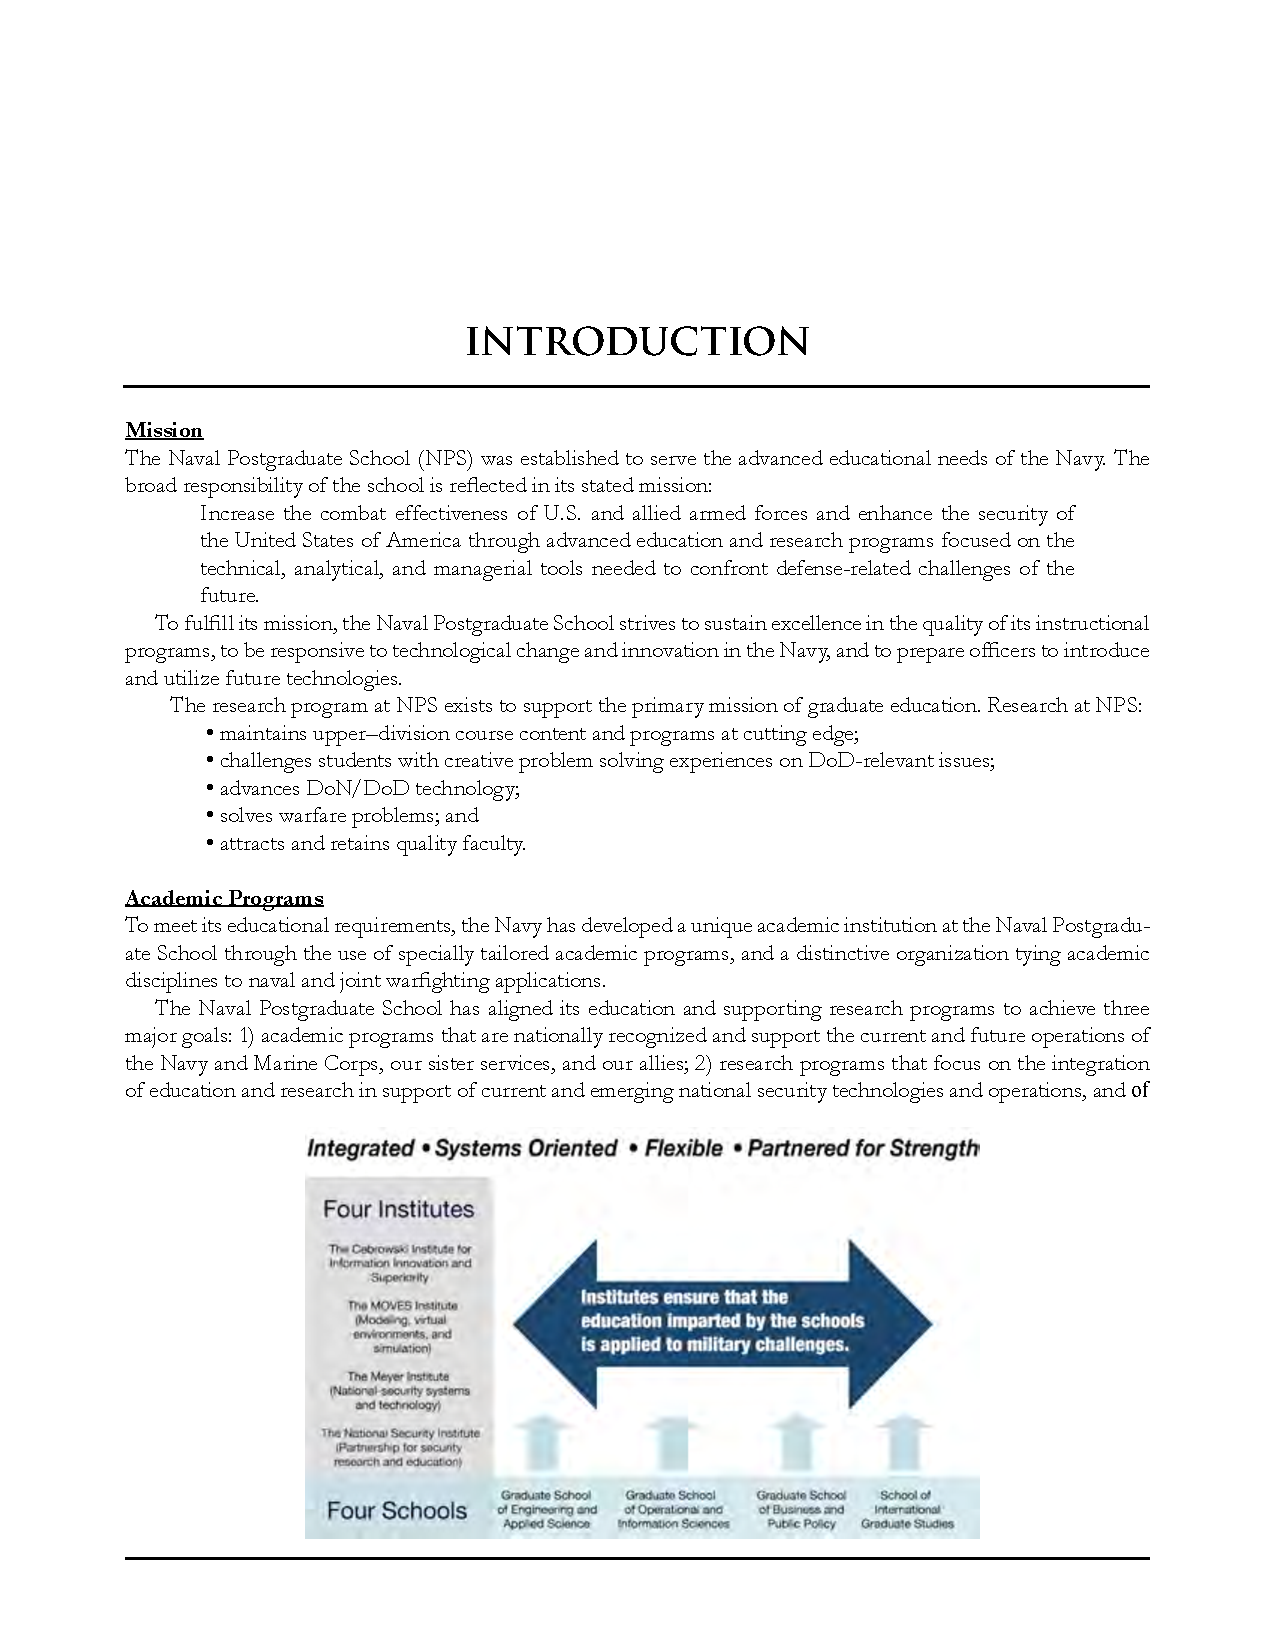
\includepdf[pages=-]{sect-frontmatter.pdf}  % INTRODUCTION
% !TEX root = report.tex

%
% TOC
%
%% Styling the TOC
%% http://hstuart.dk/2007/05/26/styling-the-table-of-contents/
%%
%% for Fancy Header documentation:
%% ftp://www.ctan.org/pub/tex-archive/macros/latex2e/contrib/fancyhdr/fancyhdr.pdf

\chapter*{\sc Table of Contents}
\renewcommand{\leftmark}{TABLE OF CONTENTS} % add manually to \leftmark
\def\contentsname{}          % don't need a name, since its in the chapter name
\vspace{-1in}                % remove some of the space after the chapter heading


\setcounter{tocdepth}{3}

%
% NPS report uses 'titletoc' package
% http://www.ctex.org/documents/packages/layout/titlesec.pdf
%
  \titlecontents{part}
  	        [25pt]                                    % left
	        {\vspace{-1.2ex}\bfseries\sc\centering}   % above
	        {\contentslabel{2.3em}}                   % before with label
	        {\hspace*{-2.3em}}                        % before without label
	        {}                                        % filler and page

  \titlecontents{chapter}
  	        [25pt]                                    % left
	        {\vspace{-1.2ex}\bfseries}                % above
	        {\contentslabel{2.3em}}                   % before with label
	        {\hspace*{-2.3em}}                        % before without label
	        {}                                        % filler and page

  \titlecontents{section}
  	        [25pt]                                    % left
	        {\vspace{-1.8ex}}                         % above
	        {\contentslabel{2.3em}}                   % before with label
	        {\hspace*{-2.3em}}                        % before without label
	        {\titlerule*[5pt]{.}\contentspage}        % filler and page


% generate first and other TOC pages
\tableofcontents
\cleardoublepage


% everything after TOC will use chapter names for left mark
\makeatletter
\renewcommand{\chaptermark}[1]{\markleft{#1}}
\makeatother
                          % toc
\NPSbody                                    % start the body
\include{thesis-dump}                       % ALL THE DATA
% !TEX root = report.tex

%
% indices
%


% TOC blank line before index
\addcontentsline{toc}{chapter}{}

% student index
\newpage
\addcontentsline{toc}{section}{\textbf{Student Index}}
\renewcommand{\leftmark}{STUDENT INDEX}
\printindex[student]

% faculty index
\newpage
\addcontentsline{toc}{section}{\textbf{Faculty Index}}
\renewcommand{\leftmark}{FACULTY INDEX}
\printindex[faculty]
                      % indices
% !TEX root = report.tex

\newpage

\addcontentsline{toc}{section}{\textbf{Obtaining a Thesis}}
\renewcommand{\leftmark}{\textsc{Obtaining a Thesis}}

\footnotesize{
NPS's Dudley Knox Library catalogs all publicly releasable theses, technical reports, and MBA professional reports. Therefore, a good source of information about what theses and various reports have been written by NPS faculty and students is the Library's general catalog, BOSUN, accessible at \url{http://www.nps.edu/Library/index.html}. An explanatory page facilitating access to NPS theses can be found at \url{http://www.nps.edu/Library/Services/Special\%20Collections/NPSTheses.html} and the same information applies to many other NPS-produced reports.

Copies of the quarterly NPS publication, \textit{Compilation of Theses Abstracts}, can be found at \url{http://www. nps.edu/Research/index.html}. The annual list of technical reports can be found at \url{http://www.nps.edu/Research/Publications/TechReports.html}. Copies of unclassified theses or other reports that are publicly releasable may be purchased from either of the following agencies depending on the particular circumstances.

\vspace{1em}
Government employees, individuals affiliated with a research and development activity within the Government, or its associated contractors, subcontractors, or grantees, under current U.S. Government contract, can order from:

\vspace{-1em}
\begin{center}
DEFENSE TECHNICAL INFORMATION CENTER\\
8725 John J. Kingman Road, STE 0944\\
Fort Belvoir, Virginia 22060--2218\\
Phone: 1-800-225-3842\\
Email: msorders@dtic.mil\\
URL: \url{http://www.dtic.mil/dtic/order.html}
\end{center}

\vspace{-1em}
Purchasing documents from DTIC requires registration with DTIC. However, many theses, particularly those completed recently, are available in electronic format for free at \url{http://stinet.dtic.mil}.

\vspace{1em}
Private U.S. citizens without a U.S. Government contract can purchase copies from:

\vspace{-1em}
\begin{center}
NATIONAL TECHNICAL INFORMATION SERVICE\\
U.S. Department of Commerce\\
5285 Port Royal Road\\
Springfield, Virginia 22161\\
Phone: 1-800-553-6847\\
Email: orders@ntis.fedworld.gov\\
URL: \url{http://www.ntis.gov/help/ordermethods.asp}
\end{center}

\vspace{-1em}
For those outside of the U.S., Canada, or Mexico, please see the NTIS arrangements with international cooperating organizations at \url{http://www.ntis.gov/help/cooperate.asp?loc=7-0-0}.

\vspace{1em}
Information needed to obtain a document is: 1) author, 2) title, 3) publication date, and 4) reference to the document as a Naval Postgraduate School thesis. General inquiries concerning faculty and student research at the Naval Postgraduate School may be addressed to:

\vspace{-1em}
\begin{center}
Vice President and Dean of Research\\
Code 04\\
Naval Postgraduate School\\
Monterey, California 93943--5138\\
Phone: (831) 656-2099\\
Email: research@nps.edu
\end{center}
}                   % backmatter

\end{document}

